%%%%%%%%%%%%%%%%%%%%%%%%%%%%%%%%%%%%%%%%%%%%%%%%%%%%%%%%%%%%%%%%%%%%%%%%
%
% Final Year Project Dissertation Document
% Author: Krishan Wyse
% Maintainer: Krishan Wyse
%
%%%%%%%%%%%%%%%%%%%%%%%%%%%%%%%%%%%%%%%%%%%%%%%%%%%%%%%%%%%%%%%%%%%%%%%%

\chapter{Background}

In the background, you will produce a critical summary of your background
literature.  Please do not just describe the background material that you find,
reference, by reference.  Once you have absorbed your background material, try
and write about your problem, describing any conflicting schools of thought,
existing solutions, shortcomings of existing approaches, etc., and reference
your sources accordingly.  Let your writing be supported by your literature.
Do not let the literature guide the structure of your writing.

Whatever you do, please make sure that you record your references as you go
along. Do not try to assemble your references at the end. A guide to
referencing can be found at \parencite{brunel2013ref}.

\section{Tables}

If you use tables in your dissertation, please label them, so they are included
in the list of tables.


\begin{table}[h]
  \centering
  \begin{tabular}{l | l | l | l }
    & 1 & 2 & 3 \\
    1 & 1 & 3 & 3 \\
    2 & 2 & 4 & 6 \\
    3 & 3 & 6 & 9 \\
  \end{tabular}
  \caption{A simple table.\label{tab:simple_table}}
\end{table}

\section{Figures}

Similarly, if you use tables in your dissertation, please label them, so they
are included in the list of figures.

\begin{figure}[h]
  \centering
  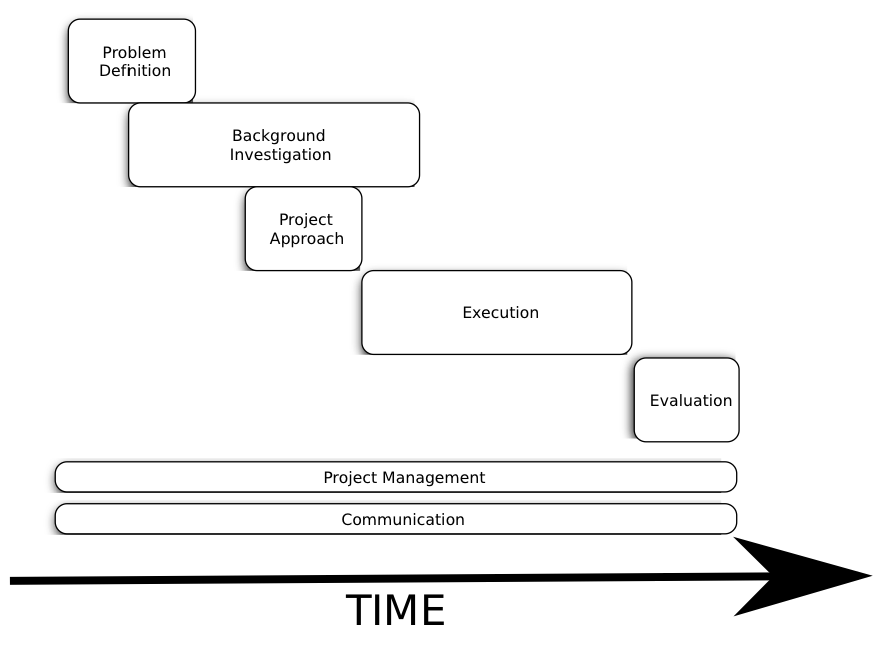
\includegraphics[width=0.5\textwidth]{fyp_model}
  \caption{A generic model of the Final Year Project\label{fig:fyp_model}}
\end{figure}
